\documentclass{article}
\usepackage[margin=2.5cm]{geometry} % Set margins
\usepackage{graphicx}
\usepackage[absolute]{textpos} % Enable absolute positioning
\usepackage{titlesec} % Package for controlling section title appearance
\usepackage[scaled]{helvet}
\usepackage[T1]{fontenc}
\usepackage{fancyhdr}
\usepackage[utf8]{inputenc}
\usepackage{lmodern}
\usepackage{amsmath}
\usepackage{url} % Load the url package
\usepackage{todonotes}

% Set up colors
\usepackage[dvipsnames]{xcolor} % Color management
% ZHAW Blue: Pantone 2945 U / R0 G100 B166
\definecolor{zhawblue}{rgb}{0.00, 0.39, 0.65}
\definecolor{zhawlightblue}{rgb}{0.82, 0.88, 0.93}

% Set up hyperref
\usepackage{hyperref}
\hypersetup{
    colorlinks=true,
    linkcolor=zhawblue,
    urlcolor=zhawblue,
    citecolor=zhawblue,
    linkbordercolor={0 0 1}
}

% Set up references
\usepackage[
    backend=biber,             % Use biber backend (an external tool)
    sorting=nyt,              % Enumerates the reference in order of their appearance
    style=apa          % Choose here your preferred citation style
]{biblatex}
\addbibresource{../../biblatex_ba.bib} % The filename of the bibliography

\usepackage[english]{babel} % Set the document language to English

\usepackage[autostyle=true, english=american]{csquotes} 
                               % Required to generate language-dependent quotes 
                               % in the bibliography

\setlength{\TPHorizModule}{1cm} % Set horizontal unit of measure
\setlength{\TPVertModule}{1cm} % Set vertical unit of measure
\setlength{\parindent}{0pt}

\renewcommand{\familydefault}{\sfdefault}

\makeatletter
\renewcommand{\maketitle}{
  \begin{flushleft} 
    \Large\textmd{\@title} 
    \par
  \end{flushleft}
}
\makeatother

% Define style of sectiontitles
\titleformat{\section}
  {\normalfont\large\mdseries}{\thesection}{1em}{}

\titleformat{\subsection}
  {\normalfont\normalsize\itshape} % Adjust style: smaller size, italic
  {} % No label
  {0pt} % Spacing between label and title
  {} % Code to execute after the title
\titlespacing*{\subsection}
  {0pt} % Left margin
  {0.8em} % Space above
  {0.2em} % Space below

% Set up fancy
\fancyhf{} % Clear all headers and footers
\renewcommand{\headrulewidth}{0pt} % Remove the header rule
\rfoot{\thepage} % Place the page number in the right footer
\pagestyle{fancy}

% Add listings package for code highlighting
\usepackage{listings}
\usepackage{xcolor}

%%%%% Title %%%%%%%%%%%%%%%%%%%%%%%%%%%%%%%%%%%%%%%%%%%%%%%%%%%%%%%%%%%%%%%%%%%%%%%%%%%%%%%%%%%%%%%%%%%%%%%%%%%%%%%%%%%

\title{Proposed Workflow for Sequence-Based Species Classification of Camera Trap Images}

\begin{document}

%%%%% Header %%%%%%%%%%%%%%%%%%%%%%%%%%%%%%%%%%%%%%%%%%%%%%%%%%%%%%%%%%%%%%%%%%%%%%%%%%%%%%%%%%%%%%%%%%%%%%%%%%%%%%%%%%
\begin{textblock}{5}(2.5,1) % Position 1cm from left and 1cm from top
  
\includegraphics[width=5cm]{resources/logo.jpg} % Add logo
\end{textblock}

\begin{textblock}{6}(13,1) % Position 14cm from left and 1cm from top
        \raggedleft
        Julian Kraft UI22\\
        Proposed Workflow V2\\
        \today
\end{textblock}

\vspace*{1.5cm}

%%%%% Document %%%%%%%%%%%%%%%%%%%%%%%%%%%%%%%%%%%%%%%%%%%%%%%%%%%%%%%%%%%%%%%%%%%%%%%%%%%%%%%%%%%%%%%%%%%%%%%%%%%%%%%%

\maketitle

\section*{Background} %%%%%%%%%%%%%%%%%%%%%%%%%%%%%%%%%%%%%%%%%%%%%%%%%%%%%%%%%%%%%%%%%%%%%%%%%%%%%%%%%%%%%%%%%%%%%%%%%

The Wildlife@Campus project is an initiative by ZHAW aimed at monitoring small mustelids in Switzerland.
One of the project's approaches involves using camera traps to collect images of the animals.
The images are captured using a camera trap box called MammaliaBox, specifically adapted for this
project \autocite{grafWildlifeCampusKleineSaeugetiere2022}.
The use of camera traps for wildlife monitoring is a well-established method \autocite{cordierCameraTrapResearch2022, 
beaudrotStandardizedAssessmentBiodiversity2016}.
Evaluating the large volume of data collected by camera traps
is a resource-intensive task, especially when approached manually. Machine learning
has proven to be a valuable tool for minimizing the workload. Several approaches exist to classify species and
detect animals in images \autocite{tabakMachineLearningClassify2019, bohnerSemiautomaticWorkflowProcess2023}.
While the most common approach is to classify single images, this project tests a sequence-based approach.

\section*{Dataset} %%%%%%%%%%%%%%%%%%%%%%%%%%%%%%%%%%%%%%%%%%%%%%%%%%%%%%%%%%%%%%%%%%%%%%%%%%%%%%%%%%%%%%%%%%%%%%%%%%%%

As part of the Wildlife@Campus project, a labeled dataset was created to train a deep learning algorithm.
The dataset is divided into seven sessions. The images are grouped into sequences, each representing a sighting
of an animal. The sequences are not standardized in length and range from 1 to 915 images per sequence.
It is worth noting that in future use cases, the sequence length will likely be more standardized.
The actual length will depend on the camera settings -- common settings such as 1, 3, 5, or 10 images per trigger --
which can be extracted from the EXIF information of the images. The dataset provides two types of labels --
the first one is not standardized and can vary between the sessions. For example scientific names and common names
are used interchangeably, and there are different spellings. The second type is a simplified and standardized version
with some visually not distinguishable species grouped together. For this project, only the simplified labels
will be used. The distribution of available sequences per label is shown in \autoref{fig:sequenceperlabel}.
The category \texttt{other} represents sequences containing more than one species, and the category \texttt{NaN}
represents sequences without a label -- both will be excluded from the from the dataset.
The category \texttt{glis\_glis} is represented in only four sequences
\todo{Is it an option to exclude this category?}, which poses a challenge to be addressed.
20\% of the sequences will be set aside for testing. A stratified split with a fixed seed will be used to ensure
reproducibility.

\begin{figure}[ht]
  \centering
  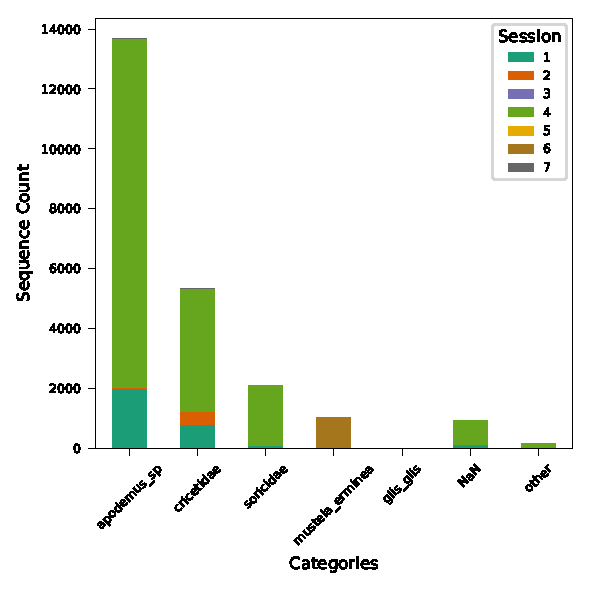
\includegraphics{resources/label2_session.pdf}
  \caption{Available sequences per label colored by session.}
  \label{fig:sequenceperlabel}
\end{figure}

\section*{Problem Statement} %%%%%%%%%%%%%%%%%%%%%%%%%%%%%%%%%%%%%%%%%%%%%%%%%%%%%%%%%%%%%%%%%%%%%%%%%%%%%%%%%%%%%%%%%%

\todo{Some of this challanges are allready addressed. I would like to discuss some of them. And is it valid to run
a first experiment and asses the results to check if the challenges are really that big of an issue?}

The problem at hand is a species classification of cameratrap images taken as sequences. The full available
information of the sequences must be used for classification. The following challenges must be addressed:

\begin{itemize}
  \item The sequences are not standardized in length.
  \item Relevant images or areas of the images must be identified.
  \item There could be multiple species in a sequence.
  \item There could be sequences with no species.
  \item The distribution of sequences per label is imbalanced.
  \item There might be objects or animals in the images not relevant for classification.
\end{itemize}

This list is not exhaustive, and further challenges may arise during the project.

\section*{General Approach} %%%%%%%%%%%%%%%%%%%%%%%%%%%%%%%%%%%%%%%%%%%%%%%%%%%%%%%%%%%%%%%%%%%%%%%%%%%%%%%%%%%%%%%%%%%

The overall idea is to create a model capable of classifying the species in a sequence of images by utilizing all 
relevant areas from each image. The model must therefore handle sequences of input images with varying lengths.
This will be achieved by processing all relevant areas individually and extracting a standardized feature array from 
each. These feature arrays will be combined using average pooling. The resulting combined feature array
will be fed into a final fully connected layer to classify the species.

\section*{Data Preparation} %%%%%%%%%%%%%%%%%%%%%%%%%%%%%%%%%%%%%%%%%%%%%%%%%%%%%%%%%%%%%%%%%%%%%%%%%%%%%%%%%%%%%%%%%%%

The Microsoft MegaDetector (MD) is a well-established model for detecting animals in camera trap images 
\autocite{hernandezPytorchWildlifeCollaborativeDeep2024a, velezChoosingAppropriatePlatform2022,
schneiderRecognitionEuropeanMammals2024}. In this project, MD will be used to detect animals in all images
of each sequence. MD outputs a list of bounding boxes for detected animals, humans, and vehicles
along with corresponding confidence scores. All animal bounding boxes with a confidence score above a certain threshold 
-- possibly 0.5 -- will be extracted and used for classification. These n images or rather areas of images
will be resized to a fixed size, working for the model used for feature extraction. 
For training, the data will be augmented using random rotation 
and random flipping -- arguably the simplest augmentation techniques for images. 
This is a common approach to increase the variety of the
training data and improve the model's generalization \autocite{shortenSurveyImageData2019}.

\section*{Model Architecture} %%%%%%%%%%%%%%%%%%%%%%%%%%%%%%%%%%%%%%%%%%%%%%%%%%%%%%%%%%%%%%%%%%%%%%%%%%%%%%%%%%%%%%%%%

The proposed model architecture is shown in \autoref{fig:model}. The idea is to use a pretrained model 
-- as of now ResNet50 is planned -- to extract features from the selected n images.
Pretrained versions of ResNet50 have been shown to be effective in image classification tasks
\autocite{bintaislamAnimalSpeciesRecognition2023}.
In ResNet, the last layer is a fully connected layer mapping the features to the output classes 
\autocite{heDeepResidualLearning2015}, the approach to repurpose a CNN for feature extraction by removing the last
layer was demonstrated by \textcite{razavianCNNFeaturesOfftheshelf2014}.
This n extracted feature embeddings will then be combined using average pooling. \todo{I have read up on different
approaches to combine features from multiple images -- I am not sure if this is valid or if there are better
options. This might be a point to discuss.} 
This approach seems to be the most simple way to combine the
n feature embeddings into one, while solving the problem of varying sequence lengths.
The resulting feature array will be fed into a final fully connected
layer to predict the species. Since the features where extracted using ResNet50 without its final layer
mapping the features to the output classes, it is reasonable to use this layer architecture to classify the species
from the combined feature array. \todo{On this step I have not jet found a lot of information.
This might be a point to discuss.}

\begin{figure}[ht]
  \centering
  \includegraphics{resources/model_proposal.pdf}
  \caption{Visual representation of the proposed model architecture.}
  \label{fig:model}
\end{figure}

\section*{Training} %%%%%%%%%%%%%%%%%%%%%%%%%%%%%%%%%%%%%%%%%%%%%%%%%%%%%%%%%%%%%%%%%%%%%%%%%%%%%%%%%%%%%%%%%%%%%%%%%%%

For model training, the extracted animal images are processed and fed into the model. To avoid adaption of the model 
to a fixed sequence length and to increase the variety of the samples, a random number of extracts per sequence are 
sampled with replacement and fed jointly into the model. In order to optimize training performance, a possible
solution could be to standardize total number of samples per batch while keeping the number of samples per sequence
variable. A part of the pretrained ResNet model will be frozen and only later layers will be subjected
to training in order for the model to be fine-tuned for the task at hand. \todo{I have read about this concept
for transfer learning. I have a feeling this is something that might need some experience to make a good decision --
I might need some help with this.}
The model will be trained using cross-entropy loss and Adam optimizer -- both standard approaches 
in image classification. The loss function will be weighted to account for the imbalanced distribution of sequences
per label.

\section*{Hyperparameter Tuning and Cross Validation} %%%%%%%%%%%%%%%%%%%%%%%%%%%%%%%%%%%%%%%%%%%%%%%%%%%%%%%%%%%%%%%%%

For the hyperparameter tuning and cross-validation, 80\% of the dataset will be, while the remaining 20\% will be
held back for testing. From the former subset an initial stratified 80/20 split will be performed for hyperparameter 
tuning using grid search and early stopping on the validation set. With the best hyperparameters, 
a 5-fold cross-validation will be carried out to evaluate model performance.

\section*{Prediction} %%%%%%%%%%%%%%%%%%%%%%%%%%%%%%%%%%%%%%%%%%%%%%%%%%%%%%%%%%%%%%%%%%%%%%%%%%%%%%%%%%%%%%%%%%%%%%%%%

Upon training completion of every trained version of the model, the best-performing model will be loaded to predict 
the test set. The predictions will be saved for evaluation and further analysis.
For prediction, the approach will be slightly modified. Instead of sampling a random number of inputs, all relevant 
areas from each image in a sequence will be passed to the model, and data augmentation will not be applied.
This ensures that all available information is used for prediction. Since some sequences in the dataset
are quite long, a limit may be necessary to avoid memory issues.

%%%%%%%%%%%%%%%%%%%%%%%%%%%%%%%%%%%%%%%%%%%%%%%%%%%%%%%%%%%%%%%%%%%%%%%%%%%%%%%%%%%%%%%%%%%%%%%%%%%%%%%%%%%%%%%%%%%%%%%

\printbibliography

\end{document}
